% Defense slide 5: the Loschmidt echo as one visual identity
%   L(t) = <Psi0| e^{-iHt} |Psi0>  =  [space-time network]  =  [continuum strip]
% Adapted from thesis/imgs/echo_strip.tex (same conventions; the transfer-matrix
% and Trotter-row boxes are removed because E has not been introduced yet).
\documentclass[tikz,border=3pt]{standalone}
\usepackage{amsmath,amssymb,braket}
\usetikzlibrary{arrows.meta,fadings}

\newcommand{\NX}{5}
\newcommand{\DX}{0.96}
\newcommand{\DY}{0.60}

\definecolor{tnbulk}{RGB}{86,196,229}
\definecolor{tncool}{RGB}{240,224,178}
\definecolor{tnrow}{RGB}{150,60,150}

\begin{document}
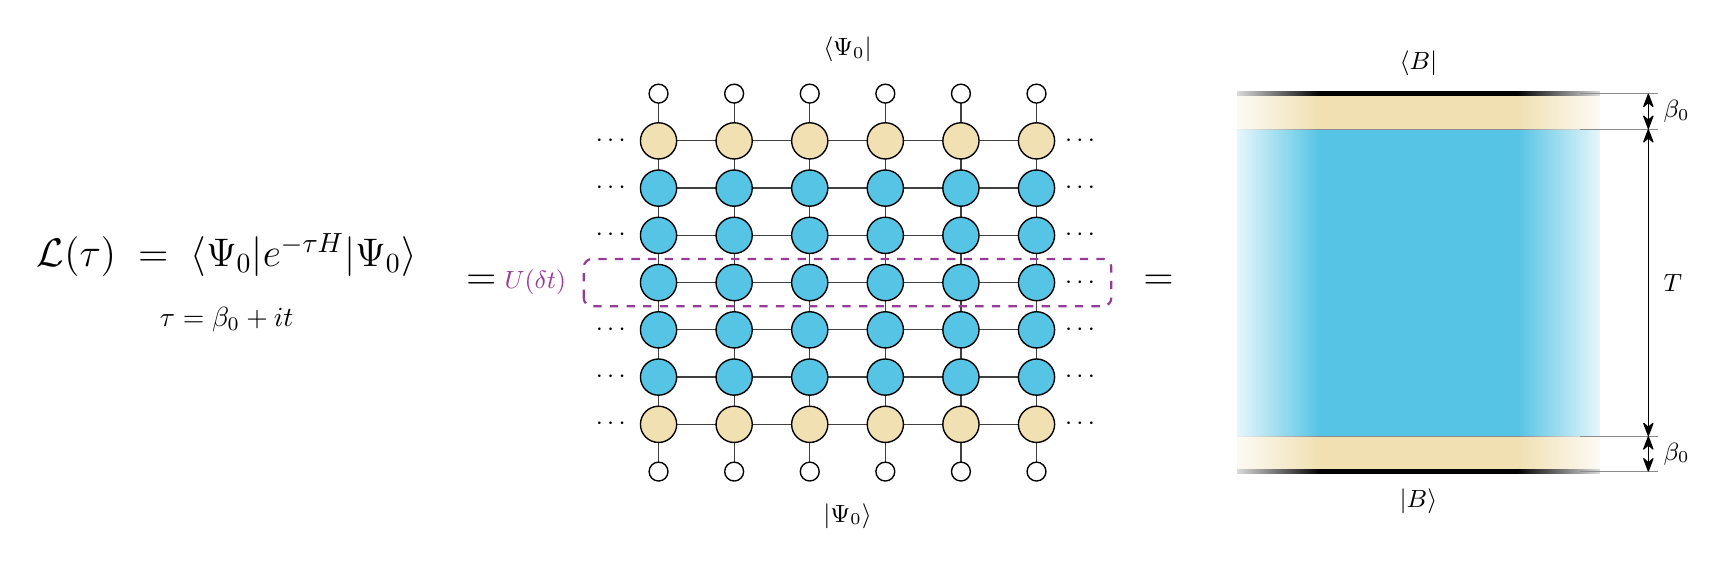
\begin{tikzpicture}[
    >={Stealth[round,length=2.0mm]},
    leg/.style={draw=black!75, line width=0.45pt},
    W/.style={circle, draw=black, fill=tnbulk, line width=0.5pt, minimum size=4.6mm, inner sep=0pt},
    B/.style={circle, draw=black, fill=tncool, line width=0.5pt, minimum size=4.6mm, inner sep=0pt},
    P/.style={circle, draw=black, fill=white, line width=0.5pt, minimum size=2.4mm, inner sep=0pt},
    hbox/.style={draw=tnrow, dashed, line width=0.8pt, rounded corners=3pt},
    tag/.style={font=\small},
  ]

  %% ================= the formula (tau defined where it first appears) ======
  \node[font=\Large, anchor=east, align=center] (formula) at (-2.95,{4*\DY})
    {$\mathcal{L}(\tau) \;=\; \braket{\Psi_0 | e^{-\tau H} | \Psi_0}$\\[0.6ex]
     {\normalsize $\tau = \beta_0 + it$}};
  \node[font=\Large] at (-2.25,{4*\DY}) {$=$};

  %% ================= panel: the lattice network =================
  \foreach \i in {0,...,\NX} { \draw[leg] (\i*\DX,0) -- (\i*\DX,{8*\DY}); }
  \foreach \j in {1,...,7} { \draw[leg] (0,\j*\DY) -- (\NX*\DX,\j*\DY); }

  \foreach \i in {0,...,\NX} {
    \foreach \j in {1,7} { \node[B] at (\i*\DX,\j*\DY) {}; }
    \foreach \j in {2,...,6} { \node[W] at (\i*\DX,\j*\DY) {}; }
    \node[P] at (\i*\DX,0)       {};
    \node[P] at (\i*\DX,{8*\DY}) {};
  }

  % row 4's left dots are replaced by the U(dt) label of the boxed row
  \foreach \j in {1,2,3,5,6,7} {
    \node[tag] at (-0.58,\j*\DY)             {$\cdots$};
  }
  \foreach \j in {1,...,7} {
    \node[tag] at ({\NX*\DX+0.58},\j*\DY)    {$\cdots$};
  }

  % one Trotter layer: each row of the network is one factor U(dt)
  \draw[hbox] (-0.95,{4*\DY-0.30}) rectangle ({\NX*\DX+0.95},{4*\DY+0.30});
  \node[tag, tnrow, anchor=east] at (-1.05,{4*\DY}) {$U(\delta t)$};

  \node[tag, anchor=south] at ({\NX*\DX/2},{8*\DY+0.28}) {$\bra{\Psi_0}$};
  \node[tag, anchor=north] at ({\NX*\DX/2},-0.28)        {$\ket{\Psi_0}$};

  \node[font=\Large] at ({\NX*\DX+1.55},{4*\DY}) {$=$};

  %% ================= panel: the continuum strip =================
  \begin{scope}[xshift={(\NX*\DX+2.55)*1cm}]
    \def\SW{4.6}
    \def\YA{0} \def\YB{0.75} \def\YC{7.25} \def\YD{8}

    \fill[tncool] (0,{\YA*\DY}) rectangle (\SW,{\YB*\DY});
    \fill[tnbulk] (0,{\YB*\DY}) rectangle (\SW,{\YC*\DY});
    \fill[tncool] (0,{\YC*\DY}) rectangle (\SW,{\YD*\DY});

    \draw[black, line width=1.6pt] (0,{\YA*\DY}) -- (\SW,{\YA*\DY});
    \draw[black, line width=1.6pt] (0,{\YD*\DY}) -- (\SW,{\YD*\DY});
    \draw[black!45, line width=0.4pt] (0,{\YB*\DY}) -- (\SW,{\YB*\DY});
    \draw[black!45, line width=0.4pt] (0,{\YC*\DY}) -- (\SW,{\YC*\DY});

    \fill[white, path fading=east] (-0.18,{\YA*\DY-0.12}) rectangle (1.05,{\YD*\DY+0.12});
    \fill[white, path fading=west] ({\SW-1.05},{\YA*\DY-0.12}) rectangle ({\SW+0.18},{\YD*\DY+0.12});

    \node[tag, anchor=south] at ({\SW/2},{\YD*\DY+0.10}) {$\bra{B}$};
    \node[tag, anchor=north] at ({\SW/2},{\YA*\DY-0.10}) {$\ket{B}$};

    \def\XD{\SW+0.62}
    \foreach \y in {\YA,\YB,\YC,\YD} {
      \draw[black!45, line width=0.35pt] ({\SW-0.25},{\y*\DY}) -- ({\XD+0.12},{\y*\DY});
    }
    \draw[<->] ({\XD},{\YB*\DY}) -- ({\XD},{\YC*\DY}) node[midway, right=2pt, tag] {$T$};
    \draw[<->] ({\XD},{\YA*\DY}) -- ({\XD},{\YB*\DY}) node[midway, right=2pt, tag] {$\beta_0$};
    \draw[<->] ({\XD},{\YC*\DY}) -- ({\XD},{\YD*\DY}) node[midway, right=2pt, tag] {$\beta_0$};
  \end{scope}

\end{tikzpicture}
\end{document}
